\documentclass[draft]{article}
\usepackage{enumitem}
\usepackage{graphicx}
\graphicspath{ {./design_images/} }

\title{Engine Bravo Design}
\author{Sean Groenenboom \and Seger Sars \and Siem Vermeulen \and Angel Villanueva \and Ronan Vlak} % Sets authors name
\date{\today}

\begin{document}

\maketitle % Generates the title
\newpage

\tableofcontents
\newpage

\section{Abbreviations}
% Please make sure to keep this in alphabetical order!
\begin{tabular}{c|c}
  \textbf{Abbreviation} & \textbf{Full from}                \\ \hline
  API                   & Application programming interface \\ \hline
  SDL                   & Simple DirectMedia Layer          \\ \hline
  Hz                    & hertz                             \\ \hline
  Sfx                   & Sound effect(s)                   \\ \hline
  ECS                   & Entity Component System           \\ \hline
  UI                    & User interface                    \\
\end{tabular}

\section{Architecture}
The game engine is a singleton. This will be the only singleton in the engine.

Managers contain only references to the game objects which are relevant to them. For example, the physics manager only contains references to game objects with collider or rigidbody components.
Whenever a component is added to or removed from a game object, the game object calls a function in the game engine class. This adds the game object to an update queue. This update queue is used every cycle, where the engine checks all components of the object in the queue, and adds or removes them to the relevant managers.
\textbf{\textit{Motivate why we made this choice!}}

\subsection{GameObjects Architecture}
\begin{itemize}
  \item \textbf{GameObjects} are the main objects in the engine. They can contain multiple components, and are the objects which are updated every cycle.
  \item \textbf{Components} are the parts of the GameObjects. They can be added and removed from GameObjects, and are updated every cycle
\end{itemize}
ECS is not used because the decision was made that there is too little time to create a ECS system that is efficient enough to warrant the extra work it would cost to implement it.
Instead of ECS, a more standard Object Oriented approach is used.

Components can be added and removed from GameObjects at runtime. This is done by calling the addComponent and removeComponent functions of the GameObject class.


\section{Physics Update}
Physics are updated sequentially in the normal game loop.
The physics are updated at a fixed rate of 50 Hz. This is done by checking how much time has passed since the last physics update, and then updating the physics the required amount of times to keep up with the accumulated time.

\subsection{Alternatives Considered}
\begin{itemize}
  \item Updating physics using a deltatime. This is undesirable, because when the update frequency of the game drops, the physics will also slow down and become unreliable and prone to error.
  \item Multithreading. Not done because rendering can then copy old data and new data in a single frame. Alternative would be copying the data to physics and copying it back when physics is finished, but that would mean copying too much data back and forth per cycle.
\end{itemize}

\section{Level Manager}
The \texttt{levelManager} (state machine responsible for transitioning between scenes) is never automatically updated, it is only updated when called by a behavior script.

\section{Physics Library}
Engine bravo makes use of the Box2D library to process any physics logic within the application. Box2D is chosen due to recommendations from teachers and since it is one of the only regularly updated ans accessible 2d physics libraries.

\section{Physics Object Types (in Box2D)}
\begin{itemize}
  \item \textbf{Staticbody}: objects which can be manually moved, but are not affected by gravity, mass, etc.
  \item \textbf{Kinematic body}: has zero mass, and can be moved by applying forces to it. It is not affected by gravity.
  \item \textbf{Dynamic body}: has mass, and is affected by gravity and other forces. It can be moved by applying forces to it.
\end{itemize}

\noindent
\textbf{Usage:}
\begin{itemize}
  \item \textbf{Staticbody} is used for walls, and objects which may move but only when explicitly told to do so.
  \item \textbf{Kinematic bodies} are not used, because the gravity of a dynamic body can instead be manually set to zero.
  \item \textbf{Dynamic bodies} are used for all objects which are affected by gravity and/or other forces.
\end{itemize}

\section{GameObjects}
GameObjects can contain multiple animtors and multiple sprites, if any of them are active they will be rendered.

\section{Tilemaps}
Tilemaps can be used to create levels more easily.
Tilemaps will be parsed in the engine.
\\
The map creator that is used to create the tilemaps is Tiled.
The reason Tiled is chosen is primarily because it was recommended for this project.
Another advantage Tiled has is its extensive documentation and its ease of use.
\\
Maps created in Tiled are exported in a .tmx format, which is a type of XML file.
The engine will parse the map file using a library called Tmxlite, which was recommended in the Tiled documentation.
Required textures can be loaded using the TextureManager.
From the parsed map, the engine will create GameObjects with a sprite component.

\section{Input}
\subsection{Supported Input types}
\begin{itemize}
  \item \textbf{Keyboard input:} the engine supports all keys on the keyboard.
  \item \textbf{Mouse input:} the engine supports left, right, and middle mouse buttons.
  \item \textbf{Controller input:} the engine supports controller input, with analog values for the joysticks.
\end{itemize}

\subsection{Input class}
The input class is a singleton, and at the start of each cycle, it updates the input states.
This is done by checking the state of the input devices, and updating the input states accordingly.
After the input states are updated, the input class is responsible for checking if a key is pressed, released, or held down.
These calculations are done at the start of every cycle, and then the input states can be read from anywhere in the engine, but hopefully only used from the behavior scripts.

\subsection{Input contexts}
An input context is a state the input system can be in where it only allows certain inputs to go through.
For example, when the player is in the main menu, the input context is set to the main menu context, and only the inputs which are relevant to the main menu are allowed to go through.
And then when the player is in the game, the input context is set to the game context, and only the inputs which are relevant to the game are allowed to go through.
These contexts and inputs that are allowed can be set by the game programmer, through an config file.




\section{UI}
\begin{itemize}
  \item \textbf{Three component types:} text, button, and image.
  \item \textbf{Text rendering:} font, text content, color, and transparency are adjustable.
  \item \textbf{Button:} has an interactable flag and an onclick callback.
  \item \textbf{Image:} has a sprite and a transparency value.
\end{itemize}

\noindent
There is a separate UI manager, which is responsible for checking where the clicks are, checking if the click was on a button, and calling the onclick callback if it was.

\section{Audio}
The audio system is is responsible for playing sfx and music.
\begin{itemize}
  \item Sfx work in a 'fire and forget' way: a single function call to the AudioSource is required to start playing the sound, and it never needs to be stopped or cleaned up in any way. The engine stops playing the sfx when it is finished \footnote{Unless specified that the sound should loop}.
  \item Music can be played, stopped and adjusted while it is playing, however, just like sfc, music does not need to be manually stopped.
\end{itemize}

\subsection{Audio library}
As discussed in the research, it is best to use an audio library (rather than manually doing system calls)
, and there are many audio libraries to choose from. By trying out various audio libraries, it was concluded that
SDL Mixer is the best library to use for this engine. While it is not as extensive as other libraries,
it has the features to meet the engine requirements, and its ease of use makes it a sensible choice.

\subsection{Class diagram}
\includegraphics[width=\textwidth]{audio_class.png}
In the following subsections, the classes in this diagram are further detailed.
\subsubsection{AudioSource}
The AudioSource is a class required by the project's API, it is one of the child classes of Component.
It will therefore be owned by a GameObject, and represent either a single sfx or song.

Things to note about the AudioSource:
\begin{itemize}
  \item When creating an AudioSource, it must be explicitly stated if it is music or an sfx. This is because the AudioManager treats these differently.
  \item mPlayOnWake (required by API) indicates whether the audio source should be played when a new scene is loaded. When this is false, the audio only plays when play() is called.
  \item The x direction and velocity represent the location of the sound in the game, from left to right (x-axis).\footnote{Because the engine is made for 2D games, there is no depth (z-axis) members. Adding verticallity (y-axis) to sound is complex, and out of the scope of this project.} \footnote{The x coordinates and velocity are unrelated to the coordinate system for the game objects.}
\end{itemize}

\subsubsection{AudioManager}
The AudioManager is, similarly to the other manager classes, responsible for controlling all of the sound features in the engine.
It contains only a few basic methods, and delegates most functionality to the audio facade and audio resource manager.

\begin{itemize}
  \item The wake method is used to indicate when a new scene is loaded. This is used to play all the AudioSources set to play on wake.
  \item The mGameObjects contains references to all GameObjects which own an AudioSource. Each cycle, this list is updated by the EngineBravo (which owns the AudioManager), by calling addSound and removeSound. This way, the AudioManager does not have to manually check which objects do and do not own an audio source.
\end{itemize}

\subsubsection{AudioResourceManager}
The AudioResourceManager is intended to reduce the amount of memory the engine requires.
If the audio resource manager is not used, each game object with a sound source would load the required sound file.
When there are many game objects which all use the same sfx file, this file would be loaded into memory multpile times, which is inefficient.
To solve this, the audio resource manager is created. This class makes sure that for each path, only one sound file is loaded.
It makes use of the ComponentPathPair, to keep track of the relation between the AudioSource components and their paths.

\subsubsection{IAudioFacade}
A facade interface to make the coupling between the AudioManager and the used audio library less tight.

\subsubsection{MixerFacade}
The implementation of the audio facade interface for SDL mixer.
Because channel \footnote{what is called a channel in SDL mixer is more commonly known as a track.} management is done
manually in SDL mixer, the mChannelCount and mLastUsedChannel variables are used to determine the next available channel for playing sfx.

\subsubsection{MixerContainer}
The mixer container holds all the
SDL mixer sound files.
The string in the mSfx map is the path to the file, because that can be considered as a sort of unique id for the sound file.

\section{Transform}
Does not need an update flag when the position is changed, as a movable object is usually moving.

\section{Collider}
Has \texttt{bodyID}, which is needed for the physics.

\section{RigidBody}
Has \texttt{bodyID}, which is needed for the physics.

\section{PhysicsEngine}{
  \begin{itemize}
    \item Steps are at 50 Hz
    \item substeps are configurable by the game programmer
    \item update method gets int of the amount of steps it need to set so less data gets copied to the world class
  \end{itemize}
 }

\section{Multithreading}
Multithreading is not added to the engine as it lies out of the scope of the project.

\section{Multiplayer}
The engine will support multiplayer.
As the customer wants the engine to follow the Unity engine API, the multiplayer system wil follow the multiplayer package of unity \textbf{Netcode}.

\subsection{Multiplayer library}
Multiple libraries have been considered, for example ENet, RakNet or Boost.
The uses library is SLikeNet. This library is a continuation of RakNet, which is a well known and well documented library.
The library is also easy to use and has a lot of features that are useful for the engine.

\subsection{Class diagram}
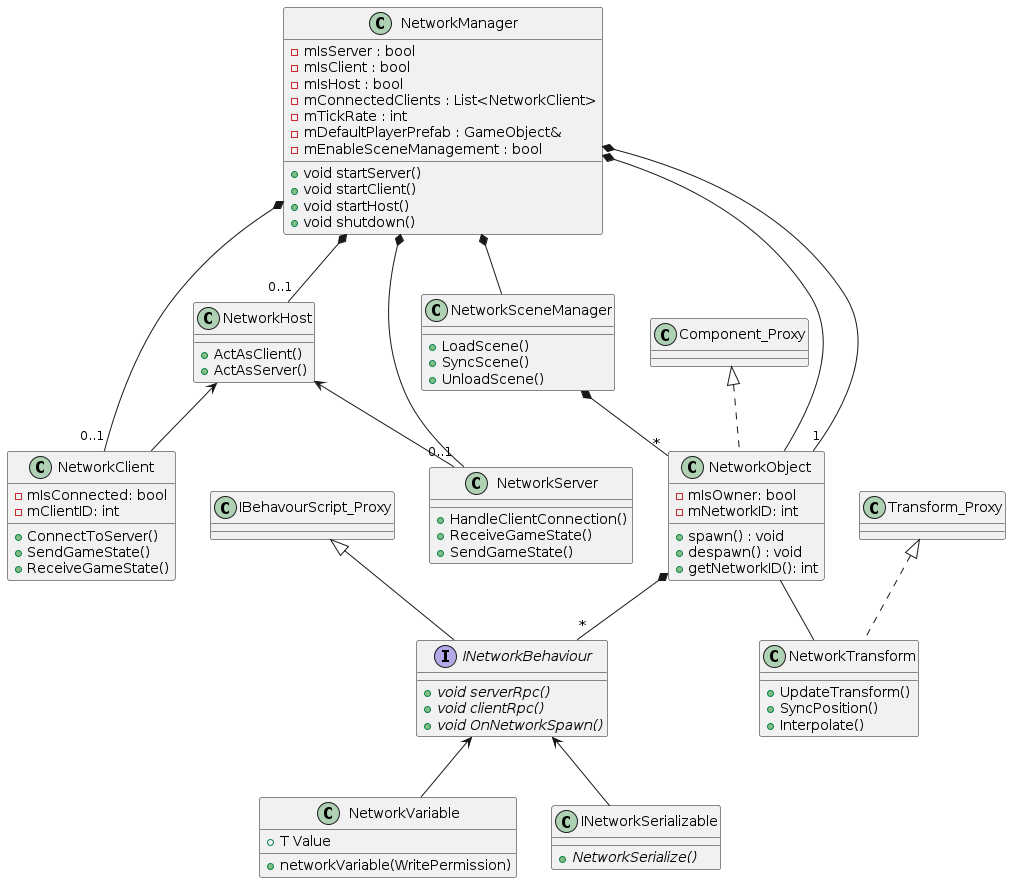
\includegraphics[width=\textwidth]{networkingClassDiagram.png}

\end{document}
